\chapter{Shape Sensitivity Analysis using Immersed Boundary Method}
In this chapter we apply the continuum sensitivity analysis to the CFD simulations conducted using the Immersed Boundary (IB) method. In this chapter the focus is on calculating the sensitivity of flow variables such as pressure and velocity to the design variable that controls the shape of the boundary, i.e. radius of a cylinder, camber of an airfoil. The boundary of the solid domain is represented using an analytical function. However, as will be shown in the following chapters this is not a required for this method. In this chapter the modifications on the IB approach to make it suitable for continuum sensitivity formulation is discussed. To the best of the author's knowledge, this is the first time that sensitivity analysis is done for CFD simulations based the continuum IB formulation.

In contrast to traditional body conformal methods, in IB approach the solid boundaries are represented by modifying the governing equation near the boundaries. In the case of continuum IB method, this is done by adding the appropriate force term to the cells adjacent to the immersed boundary. The value of these forces are calculated either using a feedback forcing \cite{goldstein1993modeling} or a penalization function \cite{arquis1984conditions}. The Navier-Stokes (NS) equations are written as shown in Equation \eqref{eq:C4_NS}.

\begin{equation}\label{eq:C4_NS}
	\frac{\partial \mathbf{u}}{\partial t} + \mathbf{u} \cdot \nabla \mathbf{u} = 
	-\frac{\nabla P}{\rho} + \mu \nabla^2 \mathbf{u} + \mathbf{f}
\end{equation}

where $\mathbf{u}$ is the velocity vector, $P$ is pressure, $\mu$ is the kinematic viscosity ($\mu / \rho$), $\rho$ is density, and $\mathbf{f}$ is the forcing term. The NS equations are solved on a Eulerian grid that is fixed in space and the IB is defined on a separate Lagrangian grid that can move. This is shown Figure \ref{fig:C4_lagrangianAndEulerianDomain}.

\begin{figure}[H]
	\centering
	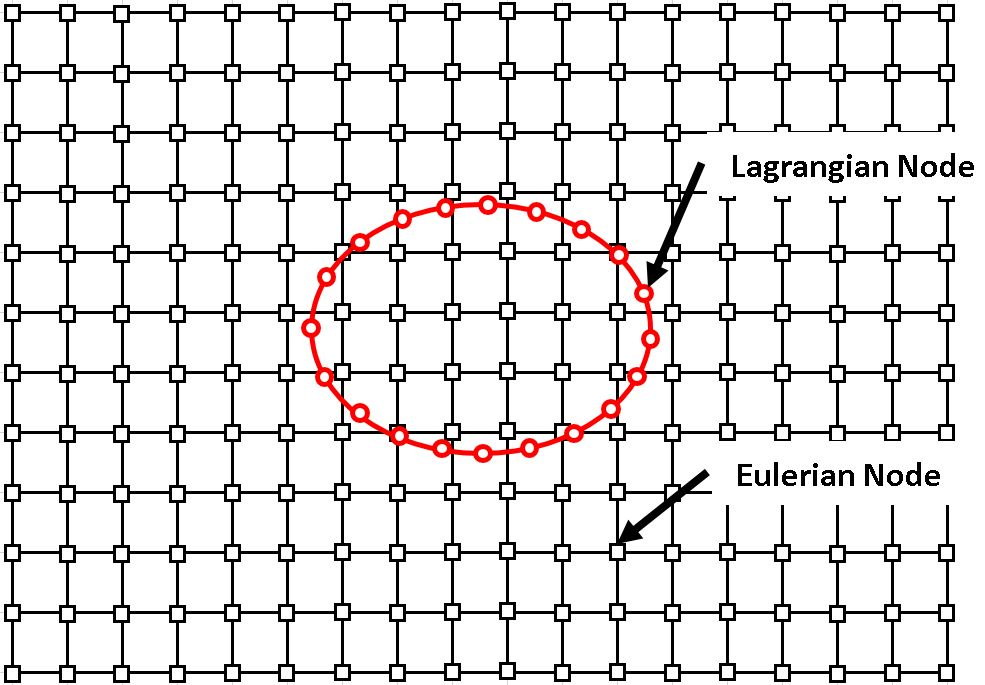
\includegraphics[width=7.00cm]{Chapter_4/figure/lagrangian_and_eulerian_nodes.jpg}
	\caption{Eulerian and Lagrangian nodes for representing the fluid and solid domain. The Eulerian and Lagrangian nodes are represented by black squares and red circles.}
	\label{fig:C4_lagrangianAndEulerianDomain}
\end{figure}

The forcing function in the penalization method is calculated at the \emph{Eulerian} nodes and is applied to computational nodes inside the solid boundary using a step function as shown in Equation \eqref{eq:C4_penalizationForcingFunction}.

\begin{equation}\label{eq:C4_penalizationForcingFunction}
	\mathbf{f} = -\mathcal{S}(\mathcal{X}(b)) \kappa \mathbf{u}
\end{equation}

where $\mathcal{S}$ is the step function, $\mathcal{X}$ defines the relative location of locations inside the domain with respect to the IB boundary, $\kappa$ is the penalization parameter, and $\mathbf{u}$ is the fluid velocity. Using this forcing function, the governing equation \eqref{eq:C4_NS} is rewritten as shown in Equation \eqref{eq:C4_NSwithPenalization}

\begin{equation}\label{eq:C4_NSwithPenalization}
	\frac{\partial \mathbf{u}}{\partial t} + \mathbf{u} \cdot \nabla \mathbf{u} = 
	-\frac{\nabla P}{\rho} + \mu \nabla^2 \mathbf{u} -\mathcal{S}(\mathcal{X}(b)) \kappa \mathbf{u}
\end{equation}

As mentioned in Chapter \ref{ch:sensitivityAnalysis}, to derive the continuum sensitivity formulation the governing equation of \eqref{eq:C4_NSwithPenalization} is differentiated with respect to the design variable, $b$. The step function $\mathcal{S}$ derivative is Dirac delta function with is singular and cannot be used to solving the governing equations in a numerical framework. Therefore a regularized Heaviside function, $\mathcal{H}$ will be employed instead of the step function for penalizing the governing equation. The effect of this function of the simulation results and sensitivity formulation will be discussed in the following sections.

In the virtual boundary method, the forcing function is calculated at the \emph{Lagrangian} nodes using Equation \eqref{eq:C3_feedbackForcingFunction}.

\begin{equation}\label{eq:C3_feedbackForcingFunction}
	\mathbf{f}(\mathbf{X}, t) = 
	\alpha \int_0^t \left[ \mathbf{u}(\mathbf{X}, \tau) - \mathbf{V}(\mathbf{X}, \tau) \right] d\tau + 
	\beta \left[ \mathbf{u}(\mathbf{X}, \tau) - \mathbf{V}(\mathbf{X}, \tau) \right]
\end{equation}

where $\mathbf{u}(\mathbf{X}, t)$ is the fluid's velocity at the Lagrangian points $\mathbf{X}$ and $\mathbf{V}(\mathbf{X}, t)$ is the desired velocity at the Lagrangian point. For the no-slip boundary condition at the solid boundary, the desired velocity $\mathbf{V}(\mathbf{X}, t)$ is zero at each of the Lagrangian points. The Eulerian nodes where the fluid's governing equation is solved does not necessary coincide with the Lagrangian points. Moreover, the forcing functions that are evaluated at the Lagrangian nodes need to tranfered to the Eulerian nodes where the governing equations for the fluid is solved. As mentioned in Chapter \ref{ch:immersedBoundary}, different mapping functions are used for transferring data between the Lagrangian and Eulerian nodes. However, none of these functions are continuously differentiable as required for the continuum sensitivity analysis. To address this issue a regularized delta function is introduced.

% ============================================================================
\section{Regularized Heaviside/Delta Function}
The Regularized Heaviside (RH) function is a step function that is smoothed so that its derivative can be calculated numerically. The RH function is also known as sigmoid function in mathematics and is characterized as a real-valued and differentiable, having either a non-negative or non-positive first derivative. There are a pair of horizontal asymptotes as $x \rightarrow \pm \infty$. The RH function is used instead of the step function to penalized the governing equation.  Several different RH functions defined in Equation \eqref{eq:C4_regularizedHeavisideFunctionFormulas} are shown in Figure \ref{fig:C4_heavisideFunctionExample}.

\begin{subequations}\label{eq:C4_regularizedHeavisideFunctionFormulas}
\begin{align}
	\mathcal{H}_1 &= \frac{1}{2} + \frac{1}{\pi} \arctan \left( x \right) \\
	\mathcal{H}_2 &= \frac{1}{1 + e^{-x}} \\
	\mathcal{H}_3 &= e^{-e^{-x}} \\
	\mathcal{H}_4 &= \frac{1 + \tanh(x)}{2}
\end{align}
\end{subequations}

\begin{figure}[H]
	\centering
	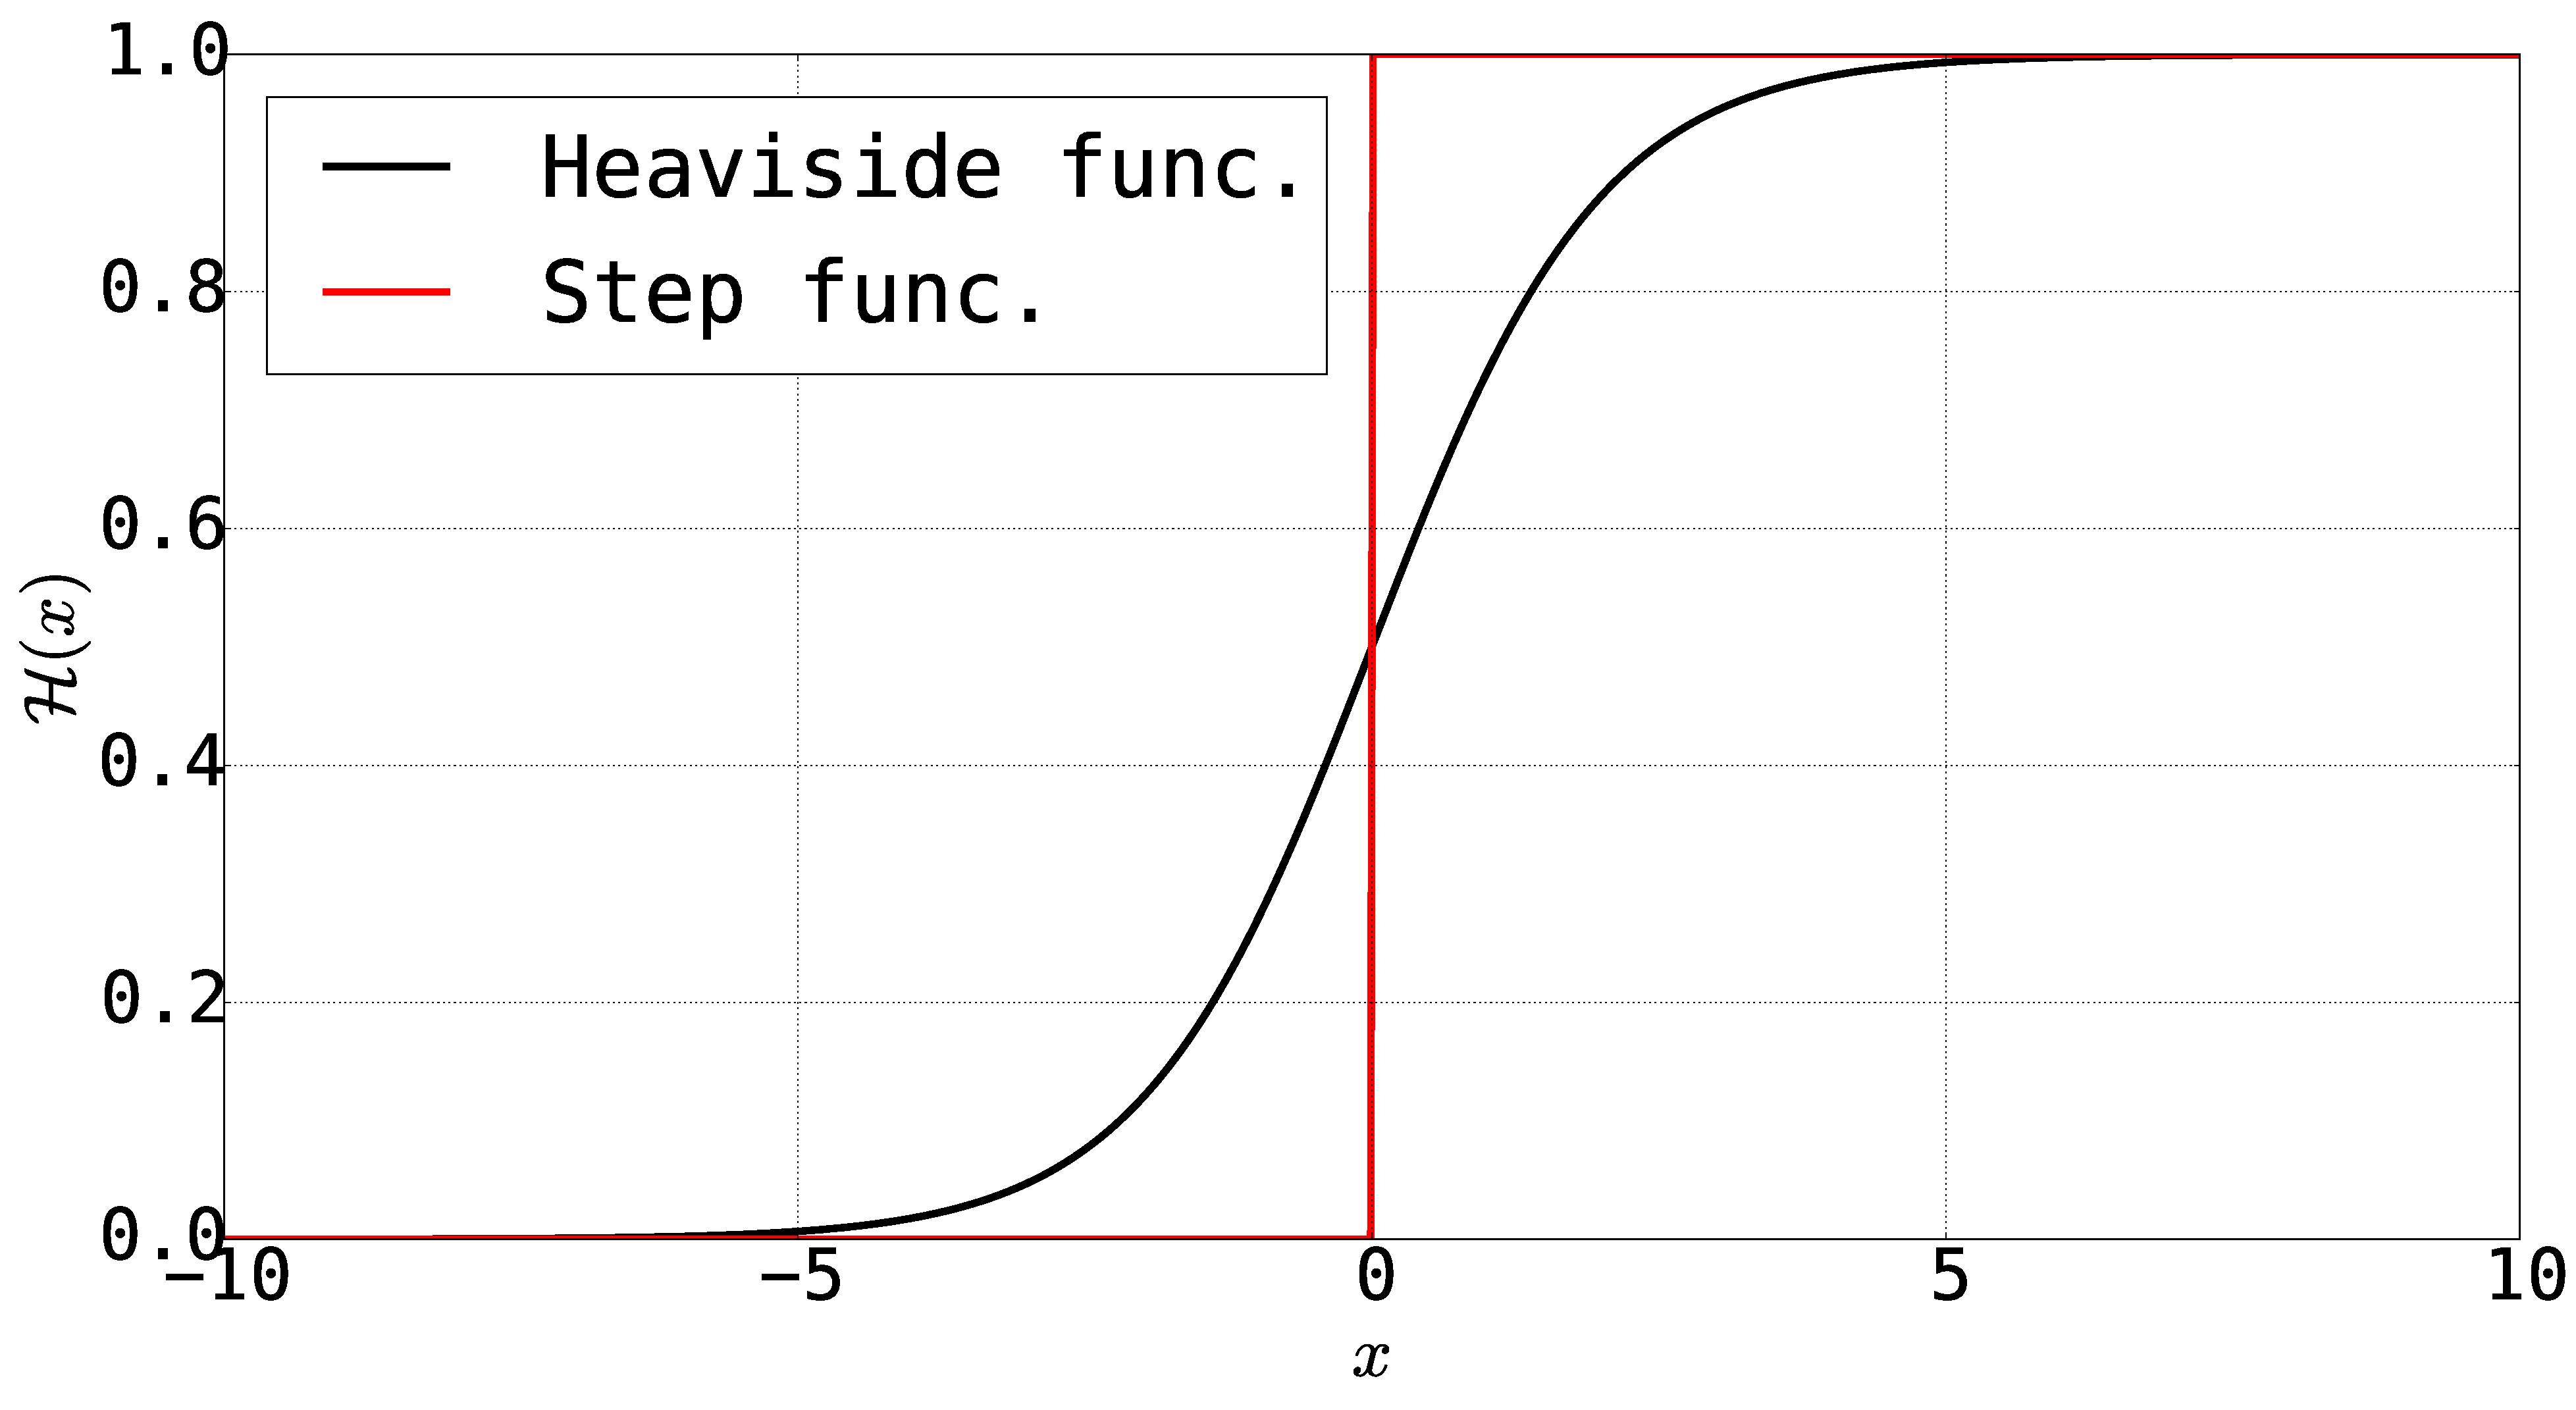
\includegraphics[width=12.00cm]{Chapter_4/figure/heaviside_function_example.eps}
	\caption{Comparison between different regularized Heaviside functions ($\mathcal{H}_i$) and step function ($\mathcal{S}$).}
	\label{fig:C4_heavisideFunctionExample}
\end{figure}

As shown in Figure \ref{fig:C4_heavisideFunctionExample}, all the RH functions are symmetric around $x = 0$ other than $\mathcal{H}_3$. This symmetry is required since the line $x = 0$ defines the boundary of the solid domain and NS equations are penalized based on the location of this boundary. In this work, the RH function is selected as $\mathcal{H}_4 = \frac{1 + \tanh(x)}{2}$ since it gives the fastest transition from $0$ to $1$. This transition is further controlled by adding the control parameter $\eta$ to the RH function definition as shown in Equation \eqref{eq:C4_heavisideFunction}. The effect of control parameter on the RH function is shown in Figure \ref{fig:C4_heavisideFunctionWithControlParamter}. As shown in Figure \ref{fig:C4_heavisideFunctionWithControlParamter} the transition region is reduced by increasing the control parameter. Using this feature, the smearing effect of penalization method can be reduced near the boundaries.

\begin{equation}\label{eq:C4_heavisideFunction}
	\mathcal{H} = \frac{1 + \tanh(x / \eta)}{2}
\end{equation}

\begin{figure}[H]
	\centering
	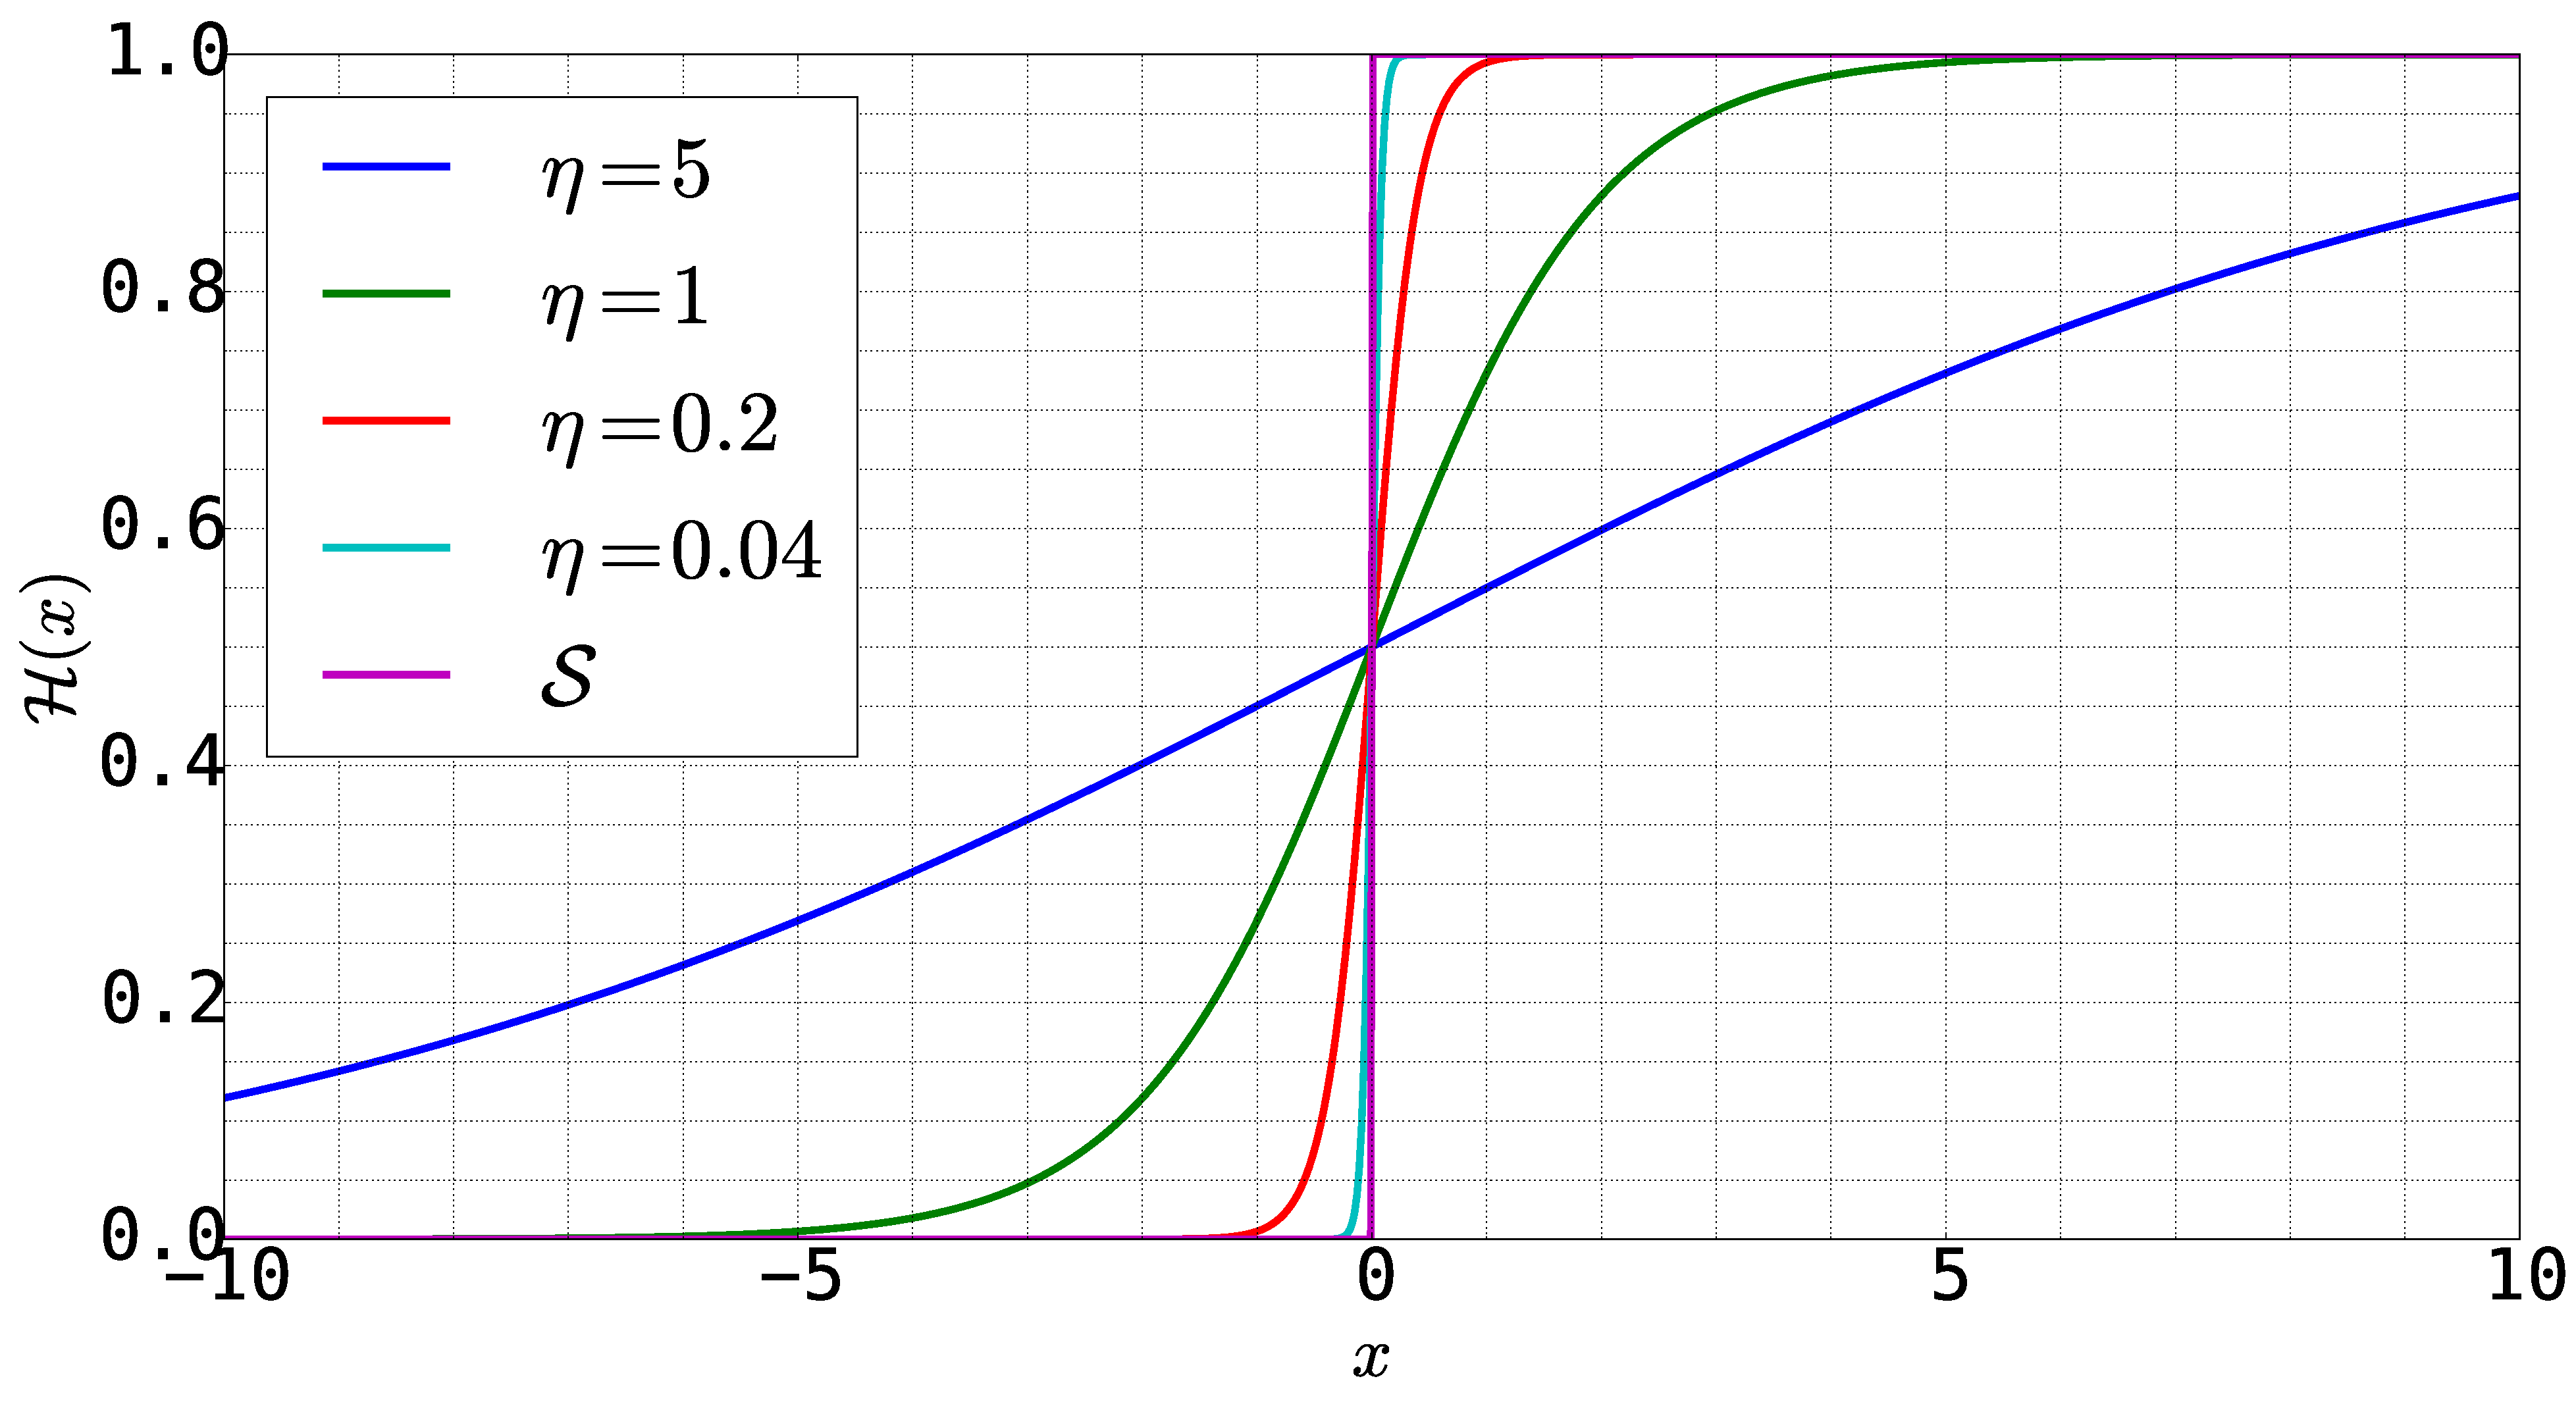
\includegraphics[width=12.00cm]{Chapter_4/figure/heaviside_function_with_control.eps}
	\caption{Effect of control parameter $\eta$ on the RH function.}
	\label{fig:C4_heavisideFunctionWithControlParamter}
\end{figure}

The penalized NS equation using the RH function of Equation \eqref{fig:C4_heavisideFunctionExample} is continuous and can be differentiated to derive the continuum sensitivity equations.

For IB simulations incorporating the virtual boundary method, the Regularized Delta (RD) function is a substitute used for transferring data between the Lagrangian and Eulerian nodes. In mathematics, the Dirac delta function is defined as the derivative of the unit step function. To be consistant with the mathematical formulation, the RD function is calculated by differentiating the RH functions of Equation \eqref{eq:C4_regularizedHeavisideFunctionFormulas} as shown in Equation \eqref{eq:C4_regularizedDeltaFunctionFormulas}. These RD functions are plotted in Figure \ref{fig:C4_deltaFunctionExample}.

\begin{subequations}\label{eq:C4_regularizedDeltaFunctionFormulas}
\begin{align}
	\mathcal{D}_1 &= \frac{1}{\pi \left(x^{2} + 1\right)} \\
	\mathcal{D}_2 &= \frac{e^{- x}}{\left(1 + e^{- x}\right)^{2}} \\
	\mathcal{D}_3 &= \frac{e^{- x}}{e^{e^{- x}}} \\
	\mathcal{D}_4 &= - \frac{\tanh^{2}{\left (x \right )} + 1}{2}
\end{align}
\end{subequations}

\begin{figure}[H]
	\centering
	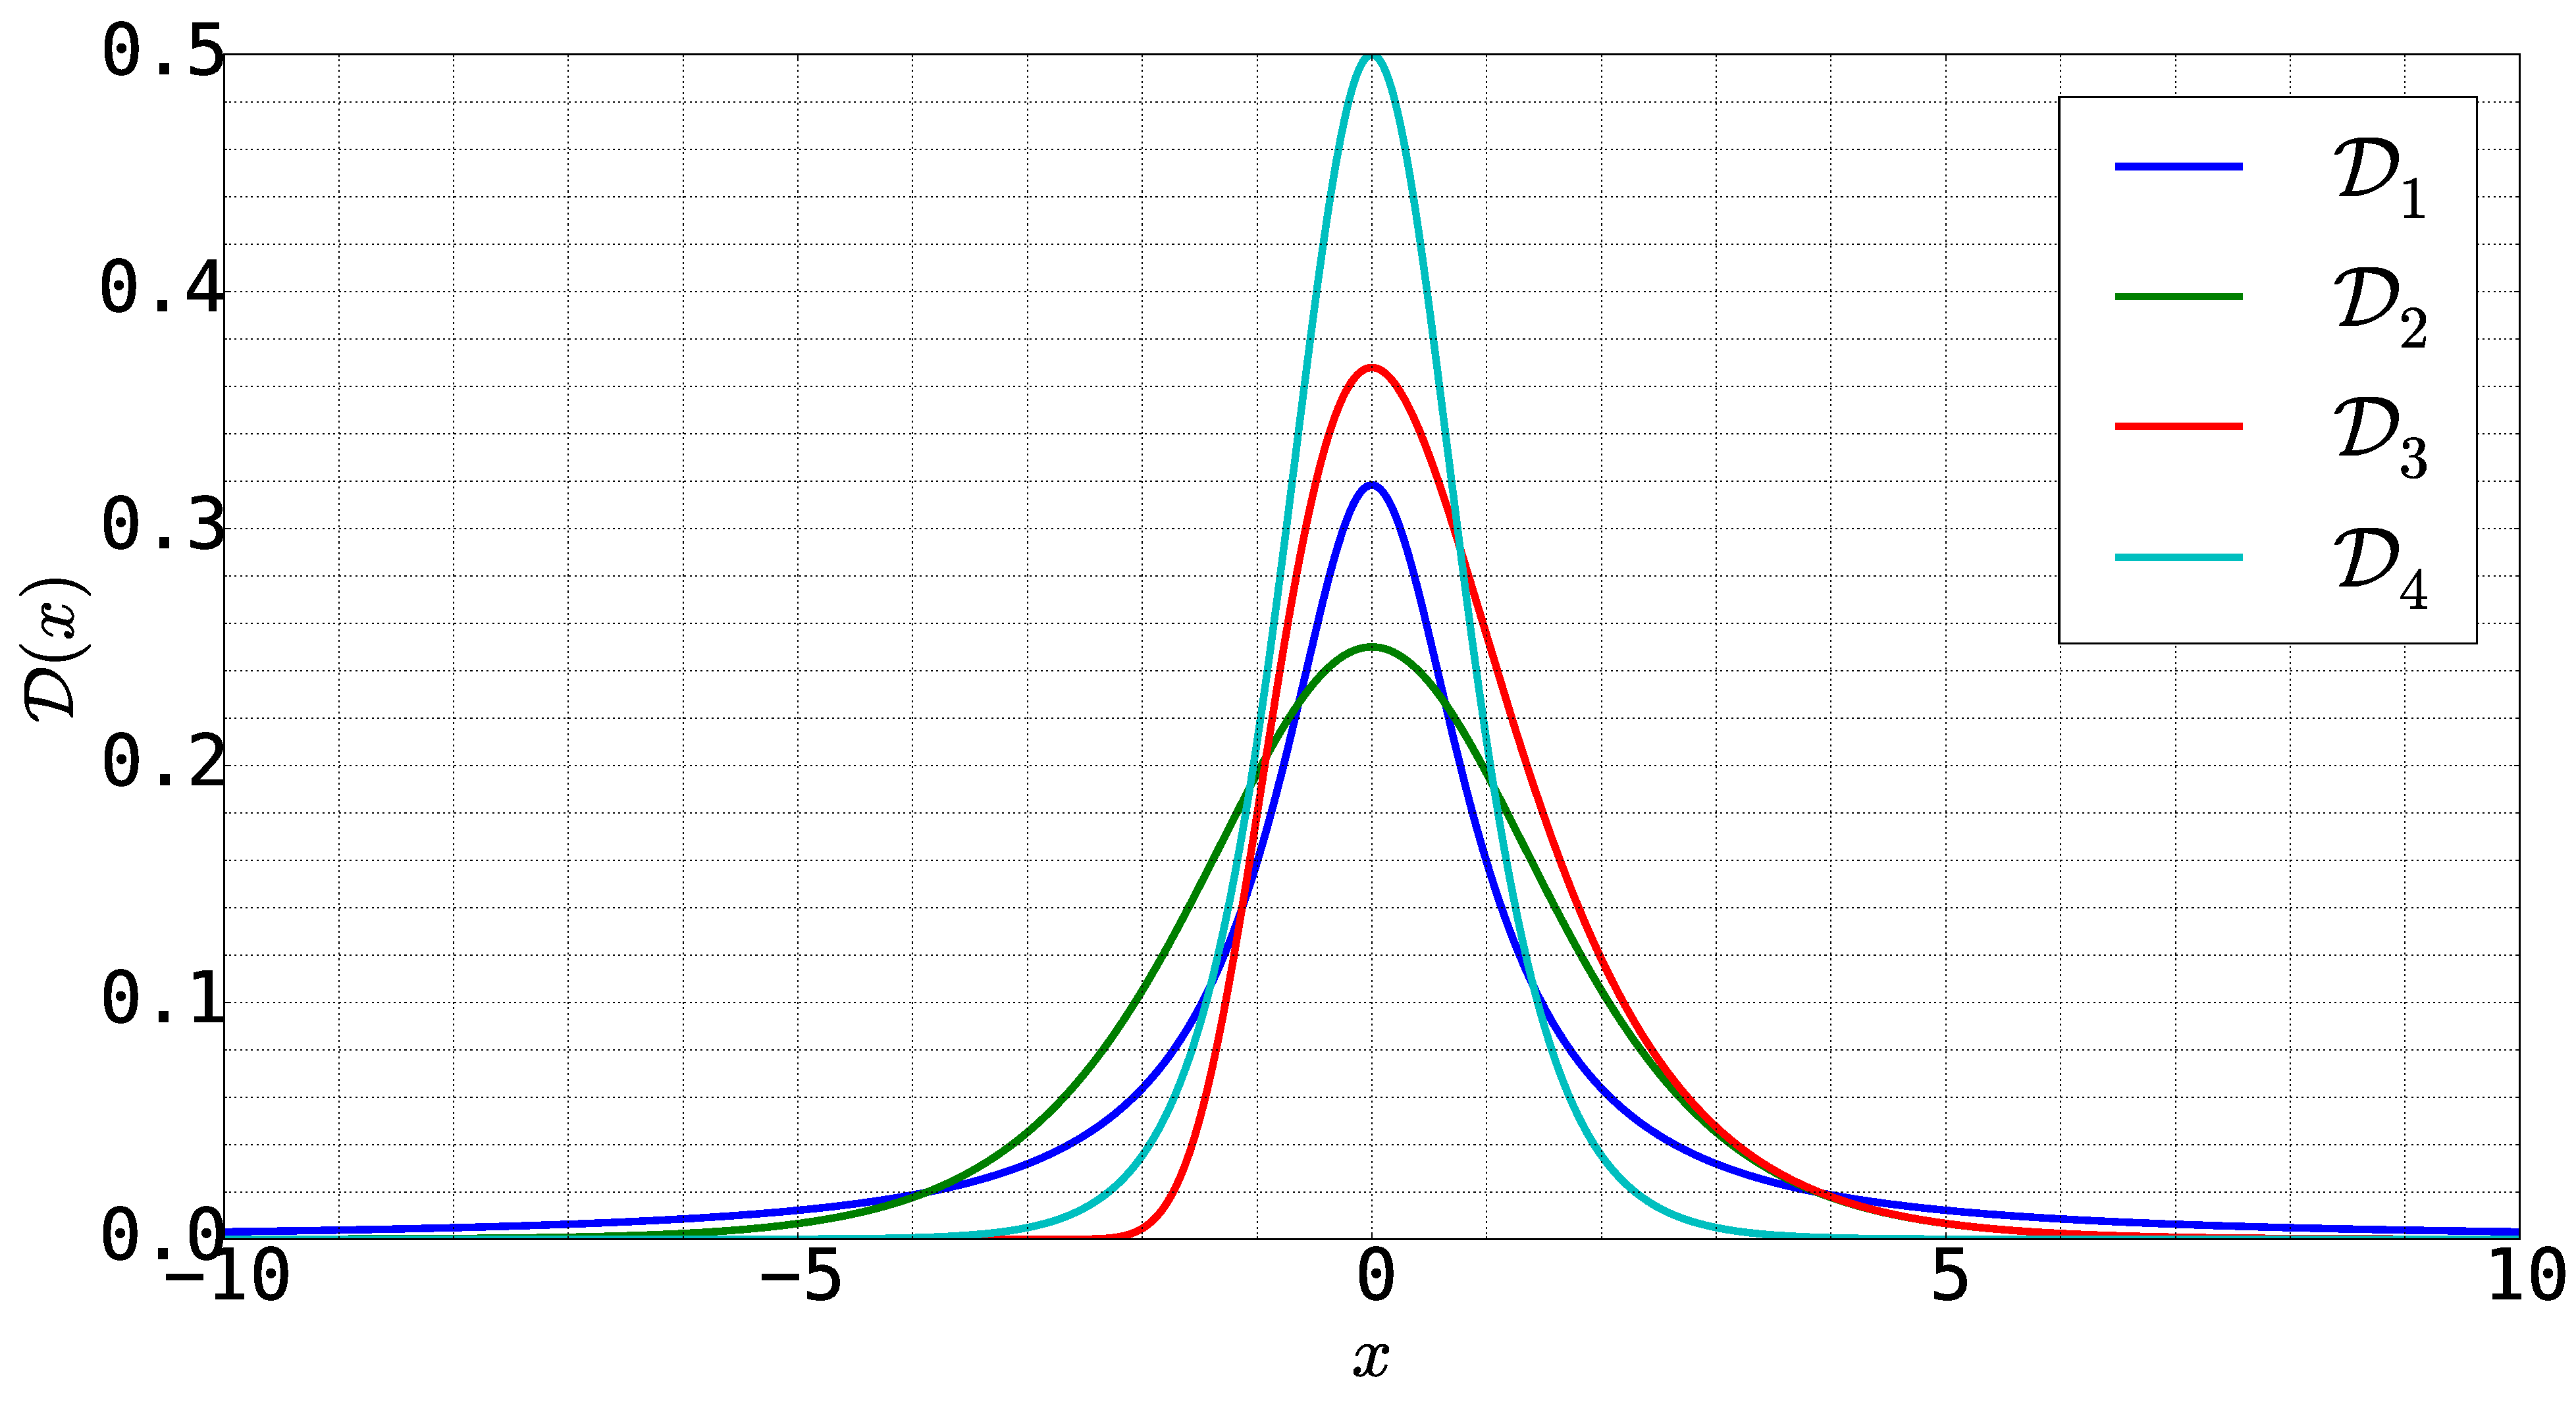
\includegraphics[width=12.00cm]{Chapter_4/figure/delta_function_example.eps}
	\caption{Comparison between different regularized delta functions ($\mathcal{D}_i$). The integral of all these functions over $x\in(-\infty, \infty)$ is equal to one.}
	\label{fig:C4_deltaFunctionExample}
\end{figure}

RD functions $\mathcal{D}_2$ and $\mathcal{D}_3$ exhibits instability issues due to different powers of exponential in the numerator and denominator and $\mathcal{D}_1$ does not have a required sharpness expected from a RD function. Therefore, in this work, the RD function $\mathcal{D}_4$ is selected for implementation in the virtual boundary method. The sharpness of this RD function is further controlled by using the $\eta$ function as used in the definition of the corresponding RH function. This is defined in Equation \eqref{eq:C4_deltaFunction}. The RD function for different value for $\eta$ is shown in Figure \ref{fig:C4_deltaFunctionWithControlParamter}.

\begin{equation}\label{eq:C4_deltaFunction}
	\mathcal{D} = \dfrac{1}{\eta} \left( \dfrac{-\tanh^{2}{\left (\dfrac{x}{\eta} \right )} + 1}{2} \right)
\end{equation}

\begin{figure}[H]
	\centering
	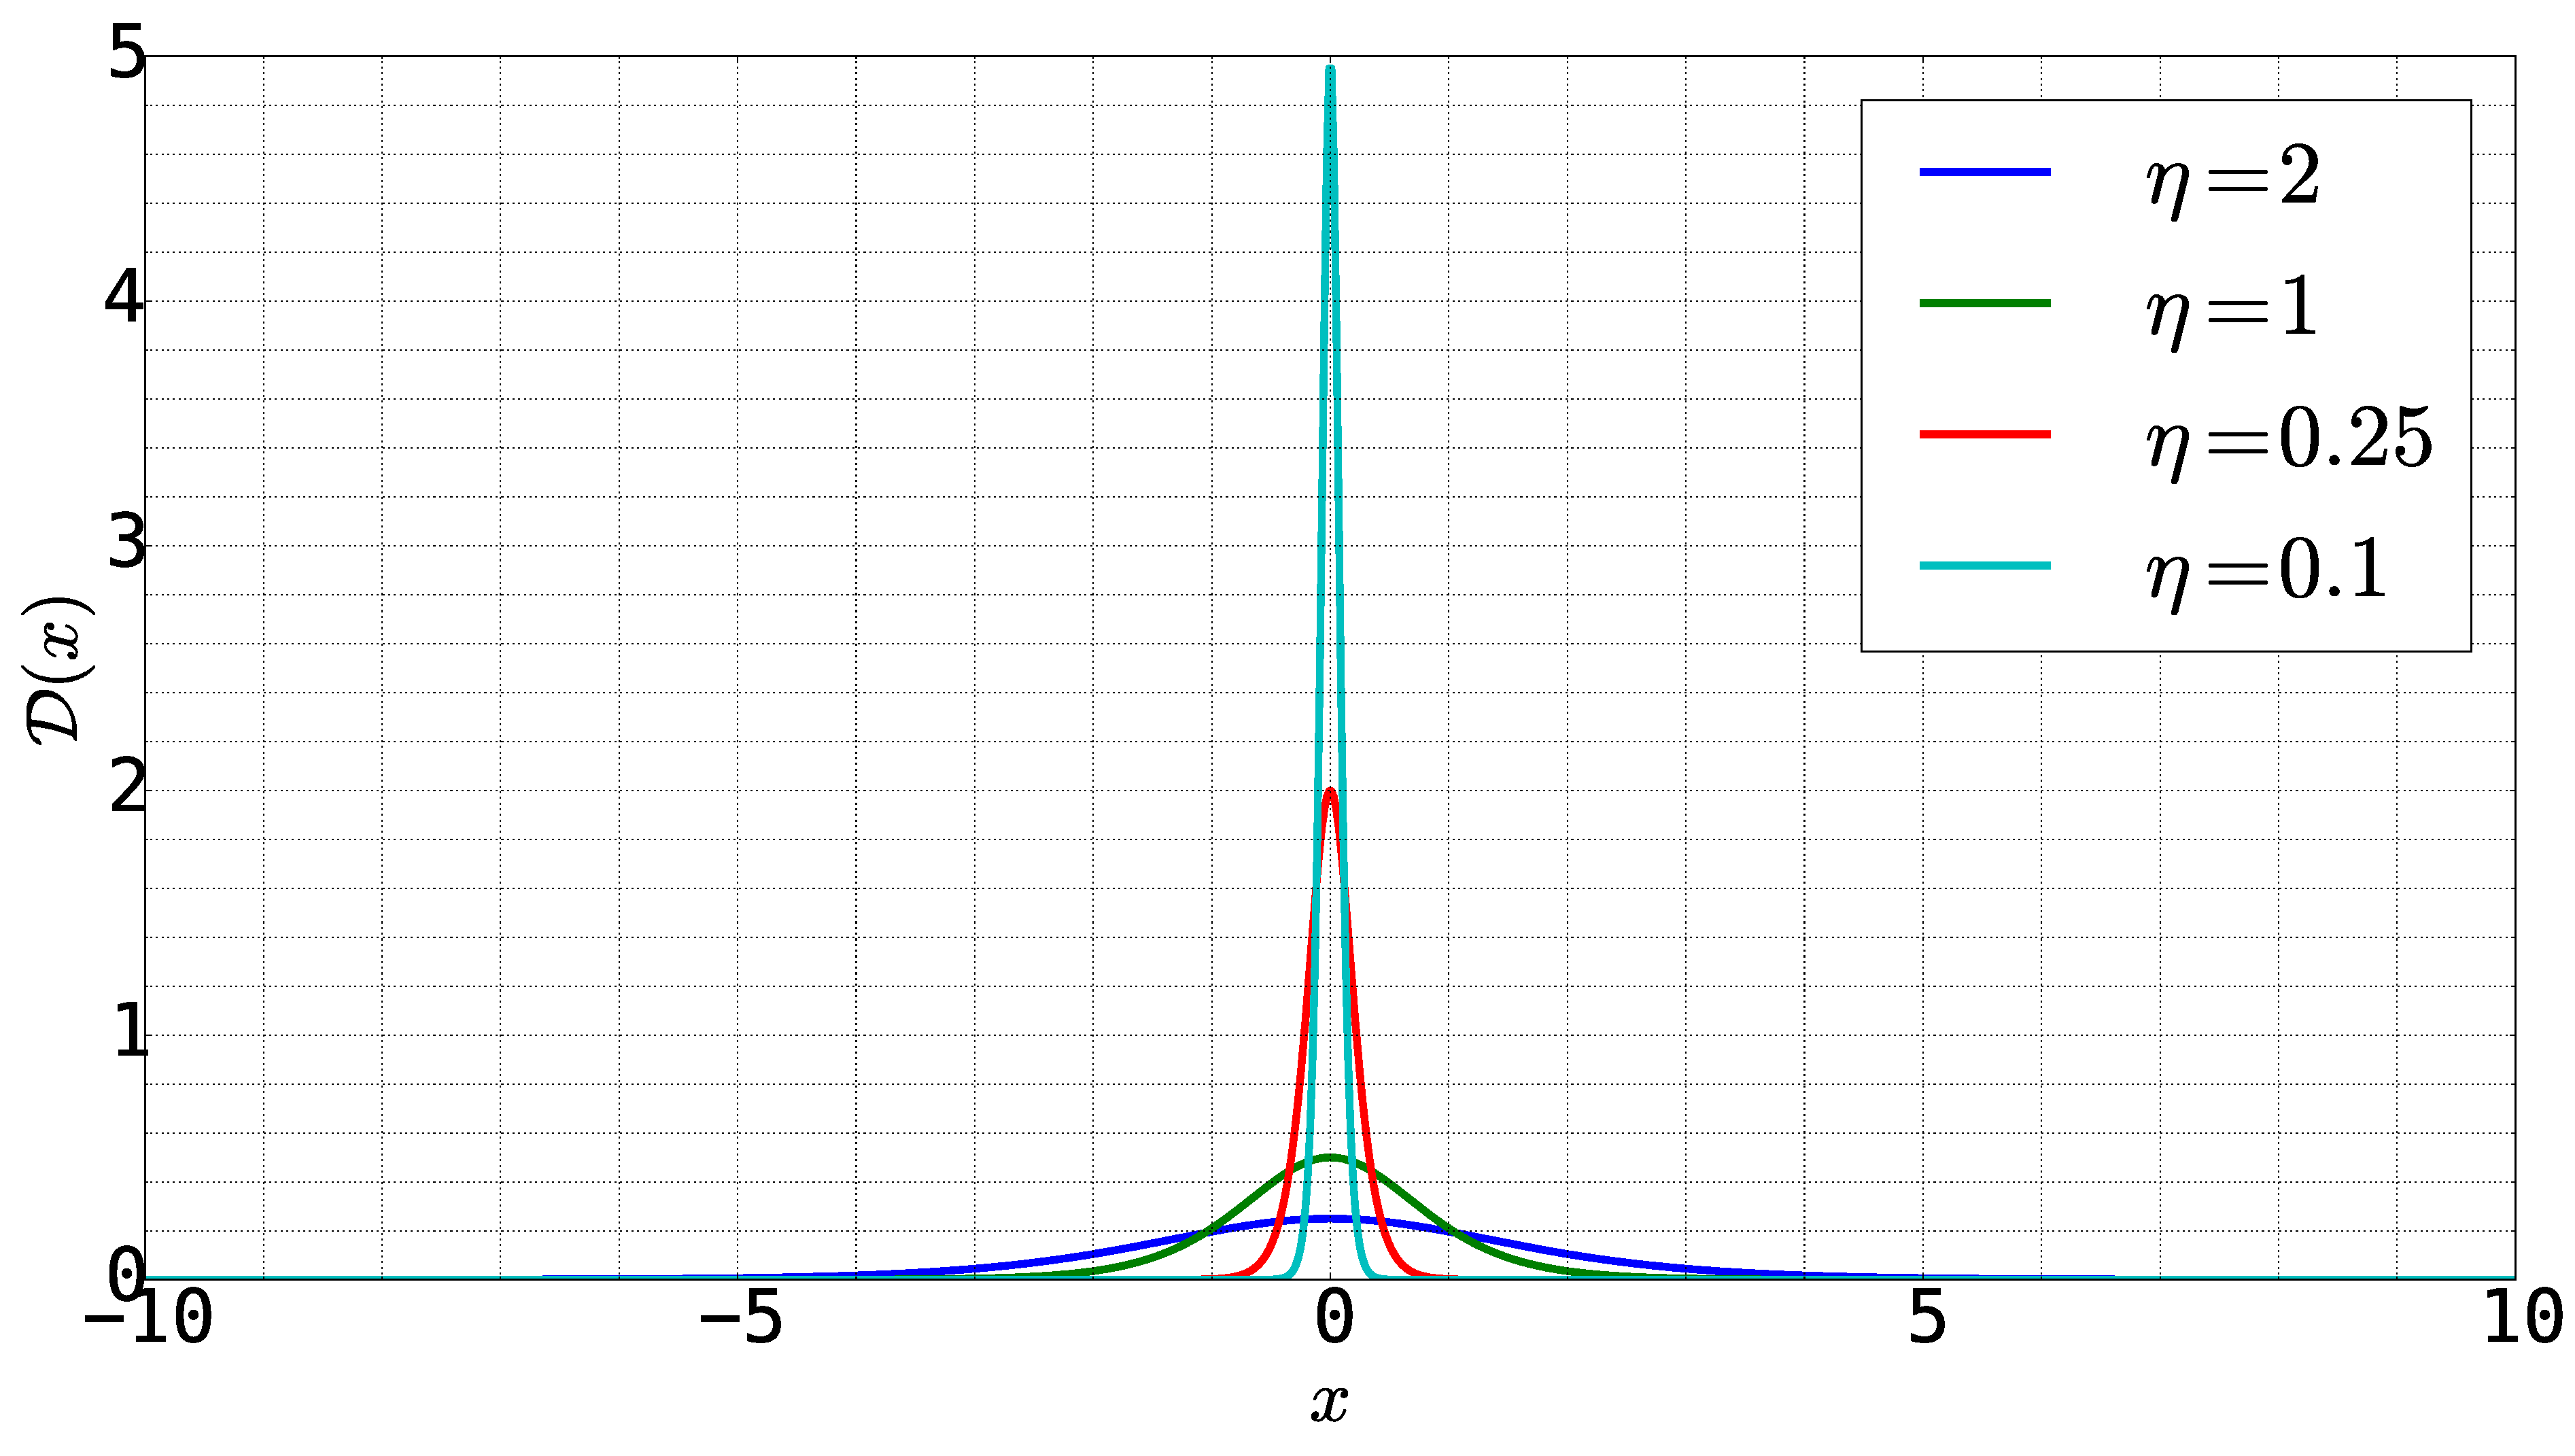
\includegraphics[width=12.00cm]{Chapter_4/figure/delta_function_with_control.eps}
	\caption{Effect of control parameter $\eta$ on the RD function.}
	\label{fig:C4_deltaFunctionWithControlParamter}
\end{figure}

As shown in Figure \ref{fig:C4_deltaFunctionWithControlParamter}, the RD function has continuous derivatives. This enables the use of virtual boundary method to be used as a part continuum sensitivity analysis for sensitivity calculation through providing differentiable governing equations.

% ============================================================================
\section{Sensitivity Analysis Formulation}
In this section, the sensitivity equations are derived for IB representation of solid boundaries. Two separate IB method are selected for the sensitivity analysis, the penalization method and the virtual boundaries method. The direct and adjoint sensitivity equations for design variables that control the shape of the IB are derived for these analysis and later applied two different demonstration problems. 

\subsection{Direct Method}
As mentioned in Chapter \ref{ch:sensitivityAnalysis}, the direct method for sensitivity analysis is preferred where the number of design variables are less than number of the functions that the sensitivities are calculated for. For this approach, the governing equations are differentiated with respect to the arbitrary shape design variable, $b$.

For the penalization method, a level-set definition of the solid boundary is used to assign penalization factors to the nodes. As defined in Chapter \ref{ch:immersedBoundary}, the boundary is defined using an analytical function $\mathcal{X}$ that depends on the shape design variable. Using the RH function, the governing equation for flow over the immersed boundaries using penalization method is written as shown in Equation \eqref{eq:C4_NSwithPenalizationIB}.

\begin{equation}\label{eq:C4_NSwithPenalizationIB}
	\frac{\partial \mathbf{u}}{\partial t} + \mathbf{u} \cdot \nabla \mathbf{u} = 
	-\frac{\nabla P}{\rho} + \nu \nabla^2 \mathbf{u} -\mathcal{H}(\mathcal{X}(b)) \kappa \mathbf{u}
\end{equation}

Equation \eqref{eq:C4_NSwithPenalizationIB} is differentiated with respect to design variable $b$ to derive the continuum sensitivity equations. The symbol $(\text{ })'$ is used instead of $\partial /\partial b$ in the sensitivity equation \eqref{eq:C4_NSwithPenalizationIBsensitivity}.

\begin{equation}\label{eq:C4_NSwithPenalizationIBsensitivity}
	\frac{\partial \mathbf{u}'}{\partial t} +
	\mathbf{u}' \cdot \nabla \mathbf{u} + \mathbf{u} \cdot \nabla \mathbf{u}' = 
	-\frac{\partial P'}{\rho} + 
	\nu \nabla^2 \mathbf{u}' - 
	\underbrace{\frac{\partial \mathcal{H}}{\partial \mathcal{X}} \frac{\partial \mathcal{X}}{\partial b} \kappa \mathbf{u}}_\text{effect of shape change} - 
	\mathcal{H}(\mathcal{X}) \kappa \mathbf{u}'
\end{equation}

Equation \eqref{eq:C4_NSwithPenalizationIBsensitivity} is solved for the velocity and pressure sensitivities ($\mathbf{u}'$, $P'$) by knowing the values of $\mathbf{u}$ from the analysis. As shown in Equation \eqref{eq:C4_NSwithPenalizationIBsensitivity}, the effect of shape change is introduced to the sensitivity equation through the derivative of the RH function. $\partial \mathcal{H}/\partial \mathcal{X}$ is easily calculated by analytical differentiating the RH function with respect to $\mathcal{X}$. The evaluation of $\partial \mathcal{X}/\partial b$ is also straight forward since it was assumed that the solid boundary is defined analytically. The boundary conditions for Equation \eqref{eq:C4_NSwithPenalizationIB} are often independent of the shape design variables. Therefore, their derivative is zero. This enables us to solve the governing Equation of \eqref{eq:C4_NSwithPenalizationIBsensitivity} for the sensitivity response.

Sensitivity implementation for the virtual boundary method is more demanding. Using the RD function, the NS equation using virtual boundary method for solid boundary definition is written as shown in Equation \eqref{eq:C4_NSwithvirtualBoundaryIB}.

\begin{align}\label{eq:C4_NSwithvirtualBoundaryIB}
	\frac{\partial \mathbf{u}}{\partial t} + 
	\mathbf{u} \cdot \nabla \mathbf{u} = 
	&-\frac{\nabla P}{\rho} + 
	\nu \nabla^2 \mathbf{u} + \nonumber \\
	&\left\{
	\alpha
	\int_0^t
	\left[
		\int \mathbf{u}(\mathbf{x}, \tau) \mathcal{D}(\mathbf{x} - \mathbf{X}) d\mathbf{x} - \mathbf{V}(\mathbf{X}, \tau)
	\right] d\tau \right.
	+ \nonumber \\
	&
	\left.
	\beta
	\int \mathbf{u}(\mathbf{x}, t) \mathcal{D}(\mathbf{x} - \mathbf{X}) d\mathbf{x} - \mathbf{V}(\mathbf{X}, t)
	\right\} \bar{\mathcal{D}}(\mathbf{x} - \mathbf{X})
\end{align}

In above equation, $\mathbf{V}(\mathbf{X}, t)$ is the desired velocity at the Lagrangian point on the solid boundary and $\int \mathbf{u}(\mathbf{x}, t) \mathcal{D}(\mathbf{x} - \mathbf{X}) d\mathbf{x}$ is the current velocity at the Lagrangian node $\mathbf{X}$ on the solid boundary calculated from the Eulerian nodes on the fluid's domain. To transfer the forces back to the Eulerian nodes, the same normalized RD function is used as shown in Equation \eqref{eq:C4_NSwithvirtualBoundaryIB} by $\bar{\mathcal{D}}(\mathbf{x} - \mathbf{X})$ where the term in the parenthesis ($\mathbf{x} - \mathbf{X}$) is responsible for casting the RD function at the location of the Lagrangian point $\mathbf{X}$. The term normalized mean that the maximum value for the RD function $\mathcal{D}$ is equal to one. This is essential to have a conservative transformation between the Eulerian and Lagrangian computational nodes. The mapping procedure is illustrated in the following example.

Assume that the analytical function $y=x^2$ is evaluated at $9$ location between $0$ and $1$. To know the function value at locations $X = 0.3321$ and $X = 0.5813$ that does not coincide with the location where the function is evaluated, it is required to use the following equation. We used the RD definition of Equation \eqref{eq:C4_deltaFunction} with $\eta = 0.1$ for this purpose.

\begin{equation}\label{eq:C4_euler2lagrange}
	y(X) = \sum_{i=1}^9 \mathcal{D}_i Y_i \Delta x_i
\end{equation}

where the subscript $i$ This equation used the data from nodes around $X$ to calculate the function value. To convert the data at $X$ (Lagrangian node) back to the surrounding nodes where the original function was evaluated, the following equation is used.

\begin{equation}
	y(x) = y(X) \bar{\mathcal{D}}(x - X)
\end{equation}

where $\bar{\mathcal{D}}(x - X)$ is a vector of numbers. The transfer of data from Eulerian nodes to Lagrangian is shown in Figure \ref{fig:C4_euler2lagrangeExample}. In this figure, the original function is represented by the solid black line and the sampling location are represented by black circles. The exact function value at the Lagrangian point is shown by red circle and the calculated value from Equation \eqref{eq:C4_euler2lagrange} is shown by blue cross. The numerical results for the comparison between the interpolated and actual values are shown in Table \ref{table:C4_euler2lagrangeExample}. The green squares represent the mapped back data to the Eulerian domain from the data at the Lagrangian point $X$ shown with red circle in Figure \ref{fig:C4_euler2lagrangeExample}. As shown here, the data at Lagrangian nodes mainly affects the two closest Eulerian nodes. The effect of Lagrangian data at $X$ decreases by moving further from $X$. The mapping from the Lagrangian to Eulerian domain has larger error compared to the mapping from Eulerian to Lagrangian grid. However, since this is done in a loop the error diminishes as simulation moves in time.

\begin{figure}[H]
	\centering
	\subfigure[$X = 0.3321$]
	{
	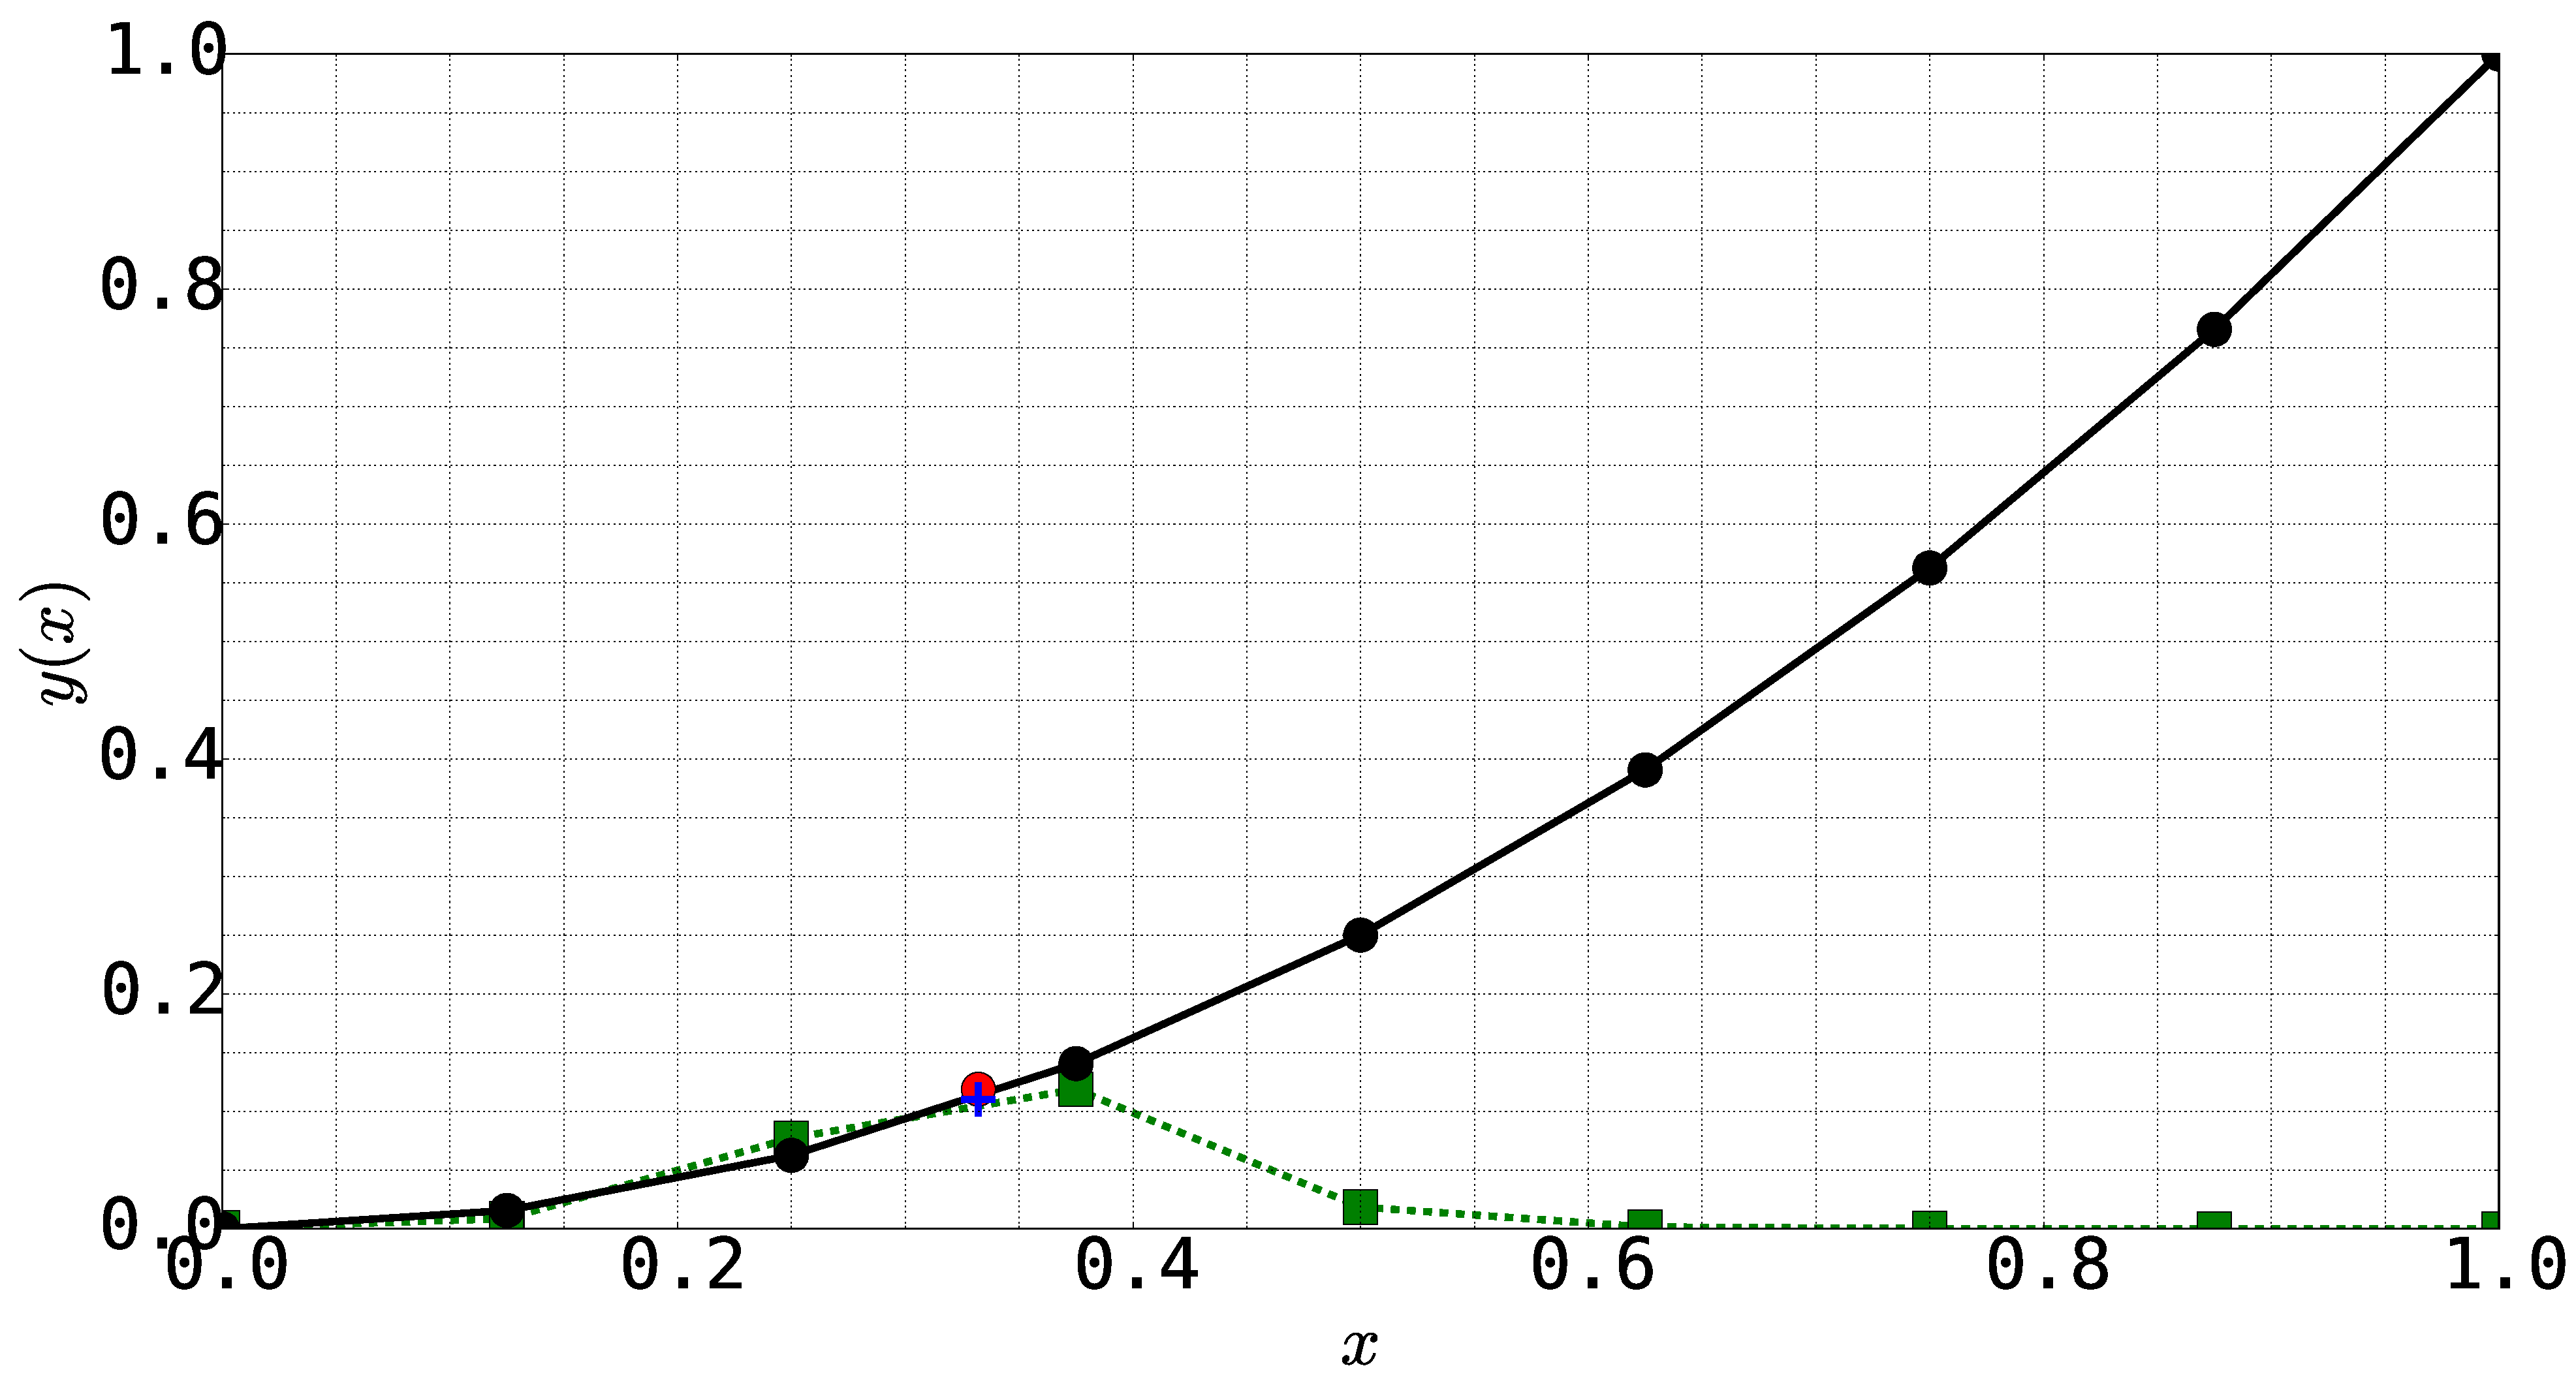
\includegraphics[width=7.0cm]{Chapter_4/figure/euler2lagrange_example_03321.eps}
	}
	\quad
	\subfigure[$X = 0.5813$]
	{
	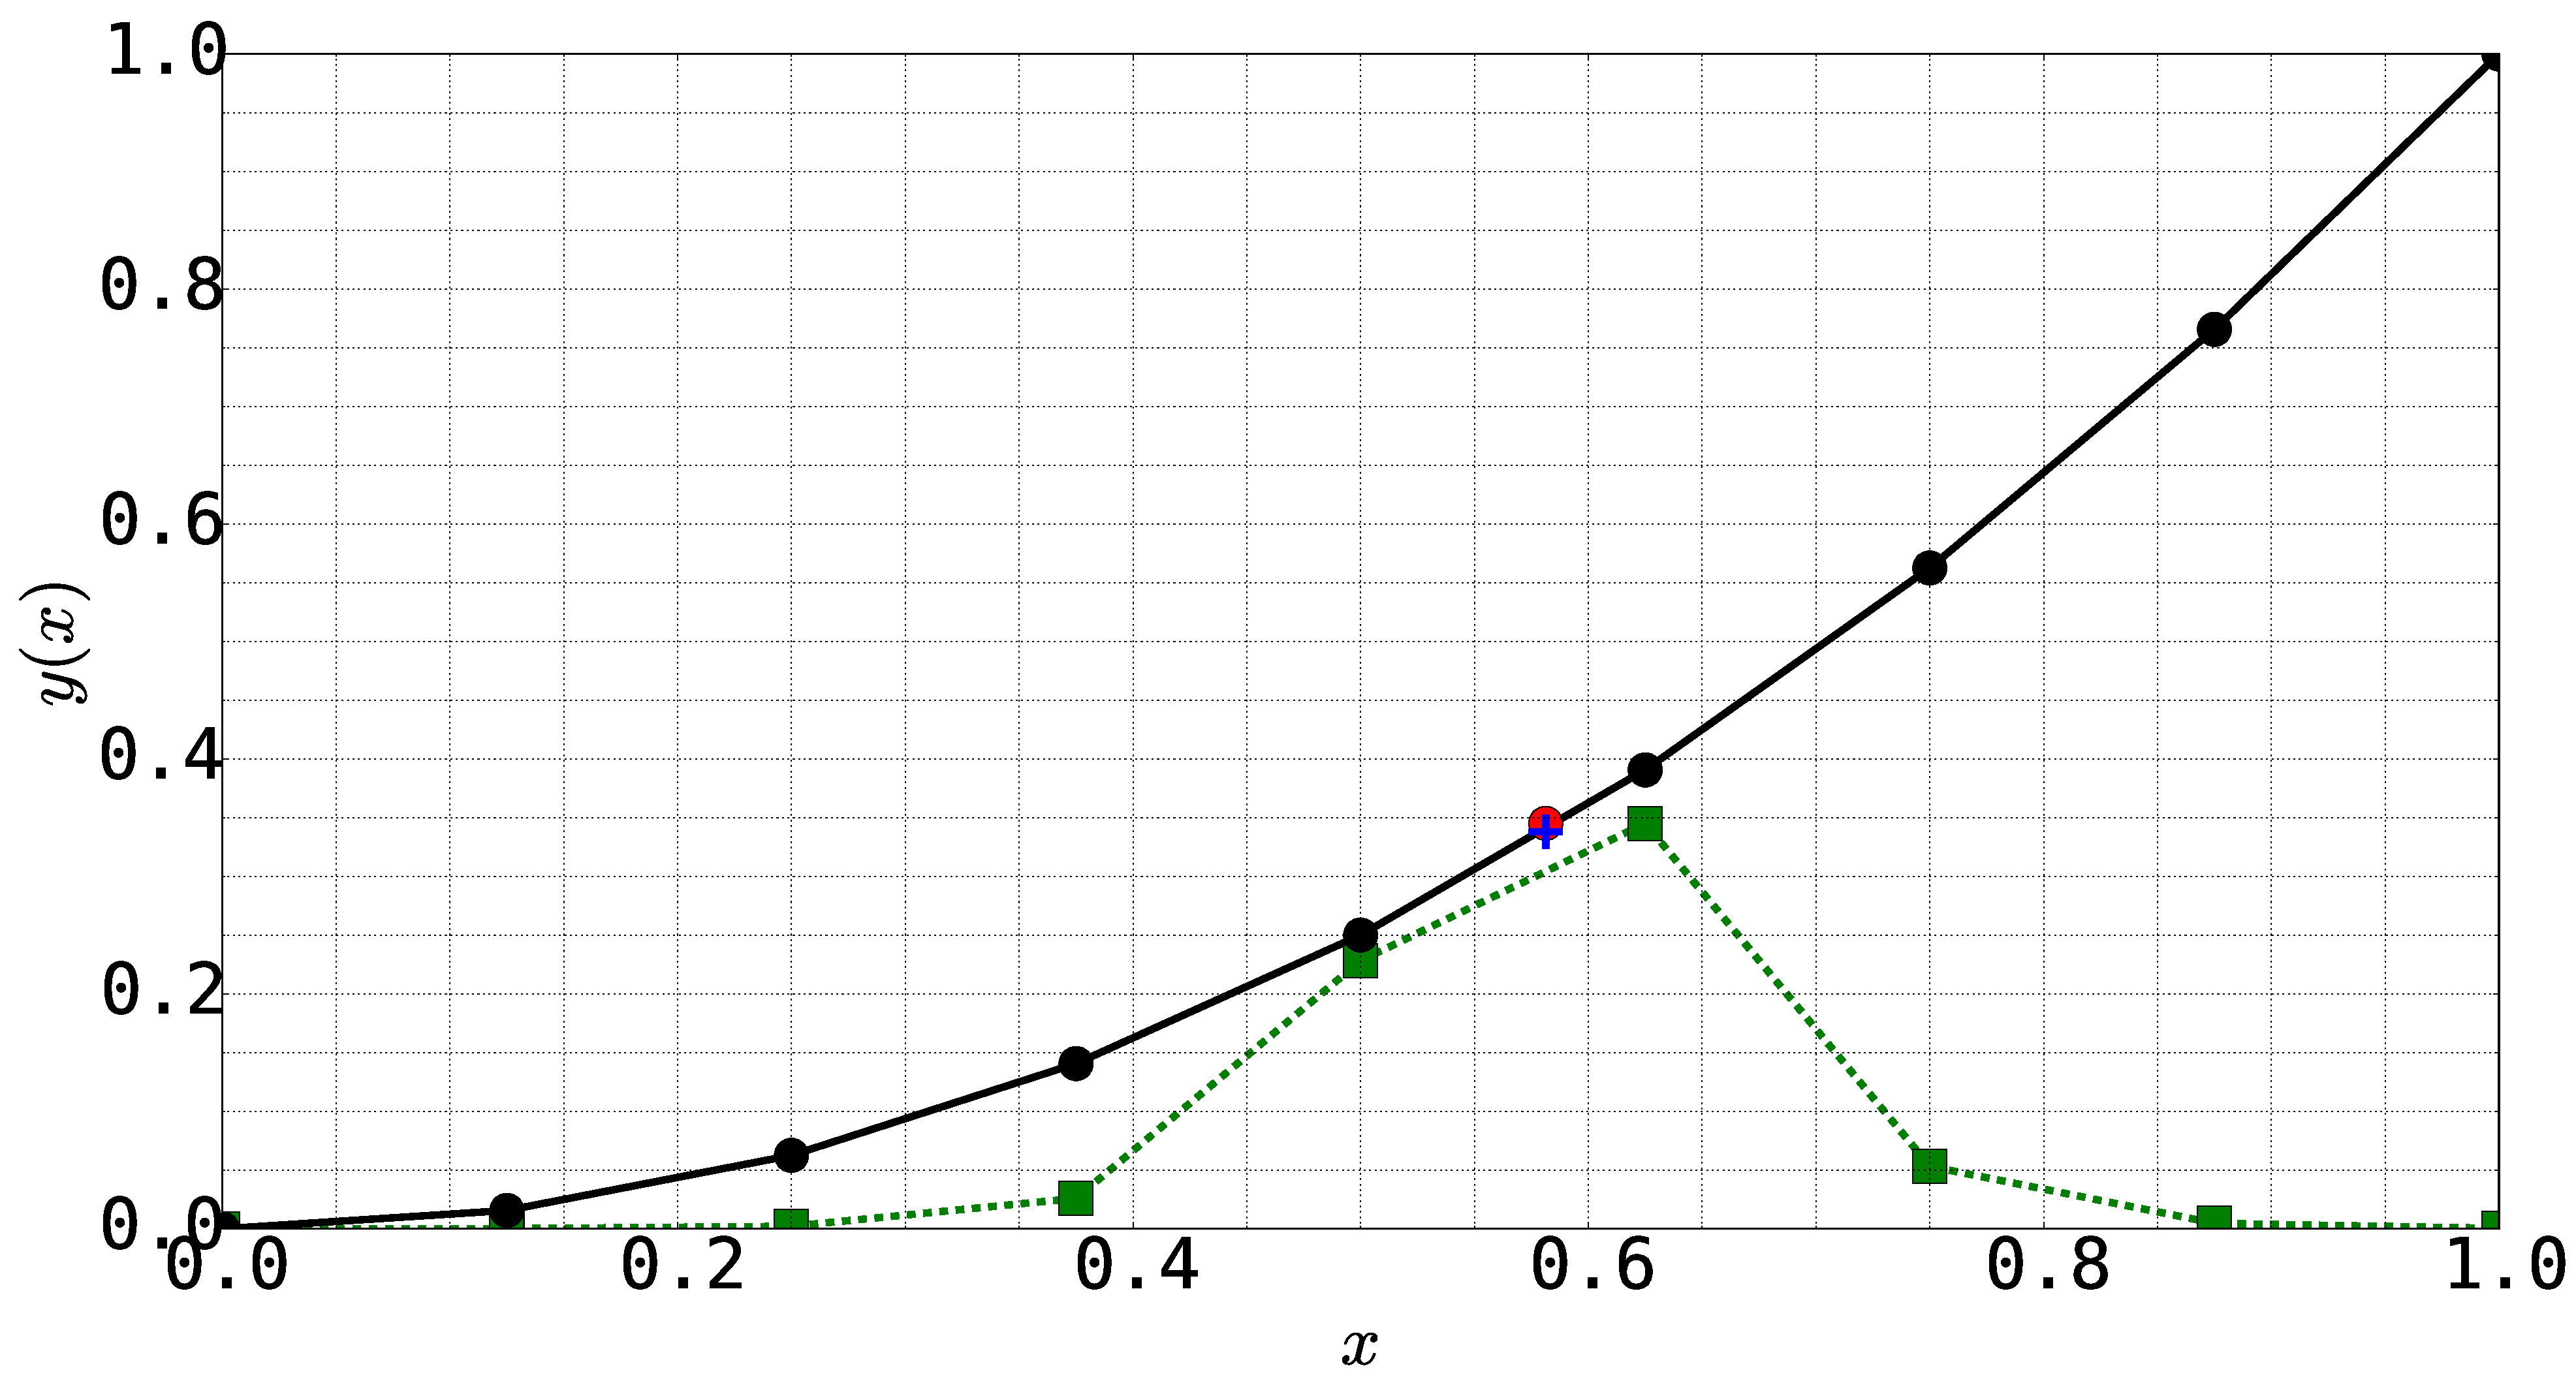
\includegraphics[width=7.0cm]{Chapter_4/figure/euler2lagrange_example_05813.eps}
	}
	\caption{Mapping the results between the Eulerian and Lagrangian computational nodes.}
	\label{fig:C4_euler2lagrangeExample}
\end{figure}

\begin{table}[H]
\centering
\begin{tabular}{| c | c |}
	\hline
	Lagrangian node location ($X$) & Absolute error \\ \hline \hline
	0.3321 & 0.0077 \\ \hline
	0.5813 & 0.0021 \\ \hline
\end{tabular}
\caption{Comparison between the true and interpolated result using the RD function at arbitrary Lagrangian location, $X$.}
\label{table:C4_euler2lagrangeExample}
\end{table}

Using this continuous mapping between the Eulerian and Lagrangian domains, the governing equation of \eqref{eq:C4_NSwithvirtualBoundaryIB} is differentiated with respect to design variable $b$ to derive the sensitivity equations. $(\text{ })'$ is used instead of the sensitivity operator, $\partial/\partial b$.

\begin{align}\label{eq:C4_NSwithvirtualBoundaryIBsensitivity}
	\frac{\partial \mathbf{u}'}{\partial t} &+ 
	\mathbf{u}' \cdot \nabla \mathbf{u} +
	\mathbf{u} \cdot \nabla \mathbf{u}' = 
	-\frac{\nabla P'}{\rho} + 
	\nu \nabla^2 \mathbf{u}' + \nonumber \\
	&\left\{
	\alpha
	\int_0^t
	\left[
		\int \mathbf{u}'(\mathbf{x}, \tau) \mathcal{D}(\mathbf{x} - \mathbf{X}) d\mathbf{x} + 
		\int \mathbf{u}(\mathbf{x}, \tau) \frac{\partial \mathcal{D}}{\partial X} \frac{\partial X}{\partial b} d\mathbf{x}
	\right] d\tau \right.
	+ \nonumber \\
	&
	\left.
	\beta
	\int \mathbf{u}'(\mathbf{x}, t) \mathcal{D}(\mathbf{x} - \mathbf{X}) d\mathbf{x} +
	\int \mathbf{u}(\mathbf{x}, t) \frac{\partial \mathcal{D}}{\partial X} \frac{\partial X}{\partial b} d\mathbf{x}
	\right\} \bar{\mathcal{D}}(\mathbf{x} - \mathbf{X}) + \nonumber \\
	&\left\{
	\alpha
	\int_0^t
	\left[
		\int \mathbf{u}(\mathbf{x}, \tau) \mathcal{D}(\mathbf{x} - \mathbf{X}) d\mathbf{x} - \mathbf{V}(\mathbf{X}, \tau)
	\right] d\tau \right.
	+ \nonumber \\
	&
	\left.
	\beta
	\int \mathbf{u}(\mathbf{x}, t) \mathcal{D}(\mathbf{x} - \mathbf{X}) d\mathbf{x} - \mathbf{V}(\mathbf{X}, t)
	\right\}
	\frac{\partial \bar{\mathcal{D}}}{\partial X} \frac{\partial X}{\partial b}
\end{align}

Equation \eqref{eq:C4_NSwithvirtualBoundaryIBsensitivity} is solved for the sensitivity response $\mathbf{u}'$, where $\mathbf{u}$ is known from the analysis results. The effect of shape change is introduced in the sensitivity equation through the derivative of the RD function, $\dfrac{\partial D}{\partial X} \dfrac{\partial X}{\partial b}$. The first term in this description is easily calculated since the RD function is known. The derivative of Lagrangian node location, $X$, to the design variable, $b$, is known since the solid boundary is defined analytically. The boundary conditions of Equation \eqref{eq:C4_NSwithvirtualBoundaryIB} are often design independent and have zero sensitivity.

\subsection{Adjoint Method}
The adjoint method is preferred when the number of the functions the sensitivity is calculated for is less than the number of design variables. To derive the continuous adjoint sensitivity, the governing equation is defined as $\mathcal{R}(\mathbf{u}, \mathbf{b}) = 0$ and the function of which the sensitivities are calculated is defined as $h(\mathbf{u}, \mathbf{b})$. In these equations, $\mathbf{u}$ is the response variable, i.e. velocity, pressure, or displacement, and $\mathbf{b}$ is the design variable. To derive the adjoint formulation, the Lagrangian is defined as shown in Equation \eqref{eq:C4_lagrangianForAdjoint}. It should be noted that if $\mathbf{u}$ satisfies the governing equation, the Lagrangian, $\Gamma$, is equal to the function of interest. Therefore, its sensitivity is equal to sensitivity of the Lagrangian.

\begin{equation}\label{eq:C4_lagrangianForAdjoint}
	\Gamma(\mathbf{u}, \mathbf{b}) = h(\mathbf{u}, \mathbf{b}) + \lambda \mathcal{R}(\mathbf{u}, \mathbf{b})
\end{equation}

Differentiating Equation \eqref{eq:C4_lagrangianForAdjoint} and rewriting the terms results in the following equation. 

\begin{equation}
	\frac{d \Gamma}{d b_i} = 
	\frac{\partial h}{\partial b_i} + 
	\left[ \frac{\partial h}{\partial \mathbf{u}} + \lambda \frac{\partial \mathcal{R}}{\partial b_i} \right]
	\frac{\partial \textbf{u}}{\partial b_i} + 
	\lambda \frac{\partial \mathcal{R}}{\partial b_i}
\end{equation}

To avoid calculating $\dfrac{\partial \textbf{u}}{\partial b_i}$, its coefficient is set equal to zero. This results in Equation \eqref{eq:C4_adjointVectorDefinition} for the adjoint variable $\lambda$.

\begin{equation}\label{eq:C4_adjointVectorDefinition}
	\lambda = -\left( \frac{\partial \mathcal{R}}{\partial \mathbf{u}} \right)^{-1} \frac{\partial h}{\partial \mathbf{u}}
\end{equation}

By knowing the adjoint vector, the sensitivity of Lagrangian function, $\Gamma(\mathbf{u}, \mathbf{b})$, is written as shown in Equation \eqref{eq:C4_functionSensitivityAdjoint}

\begin{equation}\label{eq:C4_functionSensitivityAdjoint}
	\frac{d \Gamma}{d b_i} = 
	\frac{\partial h}{\partial b_i} + 
	\lambda \frac{\partial \mathcal{R}}{\partial b_i}
\end{equation}

The adjoint formulation is implemented for a simple continuous system as defined in Figure \ref{fig:C4_stepBeamAdjoint}. The design variables are selected as the cross-sectional areas of the axial bars, $A_1$ and $A_2$. The length of bars are selected as $L_1$ and $L_2$ with a force applied at the tip, $F$. We are interested in the sensitivity of stress in bar (1) with respect to the cross-section areas $A_1$ and $A_2$.

\begin{figure}[H]
	\centering
	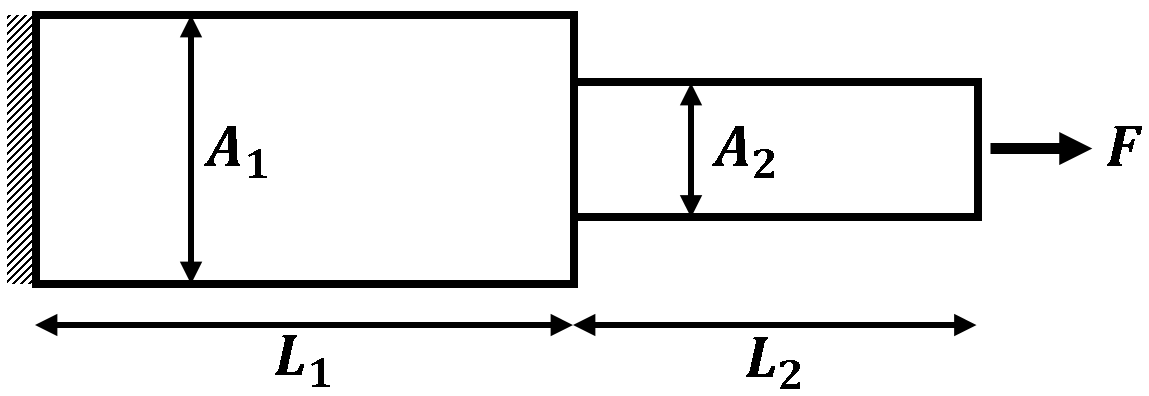
\includegraphics[width=7.00cm]{Chapter_4/figure/beam_adjoint_example_problem.png}
	\caption{Step bar problem.}
	\label{fig:C4_stepBeamAdjoint}
\end{figure}

The governing equation for this problem is defined in Equation \eqref{eq:C4_governingEquationForAdjointExample}.

\begin{equation}\label{eq:C4_governingEquationForAdjointExample}
	\mathcal{R}(\sigma, A_1, A_2) = \frac{\partial (\sigma A)}{\partial x}
\end{equation}

The solution for stress in the domain is found by integrating Equation \eqref{eq:C4_governingEquationForAdjointExample}. However, due to discontinuity at $x = L_1$, the integration is done for each section of the domain as shown in Equation \eqref{eq:C4_solutionForBarProblem}. These results agree with what is expected for the stress distribution for this problem.

\begin{subequations}\label{eq:C4_solutionForBarProblem}
\begin{equation}
	\int_0^{x < L_1} \frac{\partial (\sigma A)}{\partial x} dx = 0 \rightarrow \sigma_x A_1 - F = 0 \rightarrow \sigma_x = \frac{F}{A_1}
\end{equation}
\begin{equation}
	\int_{L_1}^{L_1 + x} \frac{\partial (\sigma A)}{\partial x} dx = 0 \rightarrow \sigma_x A_2 - F = 0 \rightarrow \sigma_x = \frac{F}{A_2}
\end{equation}
\end{subequations}

The sensitivity of the stress in the first element to the design variables, is first calculated using the direct method. This requires solving the sensitivity equation once for each of the design variables. The sensitivity equation is written by differentiating the governing equation \eqref{eq:C4_governingEquationForAdjointExample} as shown in Equation \eqref{eq:C4_sensitivityEquationForDirectMethodBar}.

\begin{equation}\label{eq:C4_sensitivityEquationForDirectMethodBar}
	\frac{\partial}{\partial x}
	\left(
	\frac{\partial \sigma}{\partial A_i} A + \sigma \frac{\partial A}{\partial A_i}
	\right) = 0
\end{equation}

The sensitivity of stress in the first bar is calculated by integrated above equation. This needs to be done for each of the design variables as shown in Equation \eqref{eq:C4_directSensitivityMethodForBarExample}.

\begin{subequations}
\begin{align}
	\int_0^x
	\frac{\partial}{\partial x}
	\left(
	\frac{\partial \sigma}{\partial A_1} A + \sigma \frac{\partial A}{\partial A_1}
	\right) dx &= 0 \nonumber \\
	\frac{\partial \sigma}{\partial A_1} A_1 + \sigma_1 &= 0 \rightarrow 
	\frac{\partial \sigma_1}{\partial A_1} = -\frac{\sigma_1}{A_1}
\end{align}
\begin{align}
	\int_0^x
	\frac{\partial}{\partial x}
	\left(
	\frac{\partial \sigma}{\partial A_2} A + \sigma \frac{\partial A}{\partial A_2}
	\right) dx &= 0 \nonumber \\
	\frac{\partial \sigma}{\partial A_2} A_2 + \sigma_2 &= 0 \rightarrow 
	\frac{\partial \sigma_2}{\partial A_2} = -\frac{\sigma_2}{A_2}
\end{align}
\end{subequations}

These results agree with the analytical sensitivity results for this problem. The Lagrangian function is defined as shown in Equation \eqref{eq:C4_lagrangianForBarExample}.

\begin{equation}\label{eq:C4_lagrangianForBarExample}
	\Gamma = h(\sigma) + \mathcal{R}(\sigma, A)
\end{equation}

where $h(\sigma)$ is the stress in first element, and $\mathcal{R}(\sigma, A)$ is the governing equation. $\mathcal{R}(\sigma, A)$ is equal to zero when the governing equation is satisfied therefore, calculating the sensitivity of $\Gamma$ is same as $h$. This is done in Equation \eqref{eq:C4_barExampleAdjointSensitivityEquation}.

\begin{equation}\label{eq:C4_barExampleAdjointSensitivityEquation}
	\frac{d\Gamma}{d \bar{A}} = 
	\frac{\partial h}{\partial \bar{A}} + \lambda \frac{\partial \mathcal{R}}{\partial \bar{A}} + 
	\left[
	\frac{\partial h}{\partial \bar{\sigma}} + \lambda \frac{\partial \mathcal{R}}{\partial \bar{\sigma}}
	\right]
	\frac{\partial \bar{\sigma}}{\partial \bar{A}}
\end{equation}

where $\bar{\text{ }}$ represents a vector. $\dfrac{\partial h}{\partial \bar{A}}$ is equal to zero since $h = \sigma_1$ and the stress does not explicitly related to the cross-sectional area. $\dfrac{\partial h}{\partial \bar{\sigma}}$ is calculated easily. $\dfrac{\partial \mathcal{R}}{\partial \bar{\sigma}}$ is calculated as shown in Equation \eqref{eq:C4_sensitivityOfGoverningEquationToStressBarExample}.

\begin{subequations}\label{eq:C4_sensitivityOfGoverningEquationToStressBarExample}
\begin{align}
	\frac{\partial \mathcal{R}}{\partial \sigma_1} &= 
	\frac{\partial }{\partial x}
	\left(
	\frac{\partial \sigma}{\partial \sigma_1} A + \sigma \frac{\partial A}{\partial \sigma_1}
	\right) \nonumber \\
	&\rightarrow
	\int_0^{L_1}
	\frac{\partial}{\partial x}
	\left(
	\frac{\partial \sigma_1}{\partial \sigma_1} A_1
	\right) dx + 
	\int_{L_1}^{L_1 + x}
	\frac{\partial}{\partial x}
	\left(
	\frac{\partial \sigma_2}{\partial \sigma_1} A_2
	\right) dx = A_1
\end{align}
\begin{align}
	\frac{\partial \mathcal{R}}{\partial \sigma_1} &= 
	\frac{\partial }{\partial x}
	\left(
	\frac{\partial \sigma}{\partial \sigma_2} A + \sigma \frac{\partial A}{\partial \sigma_2}
	\right) \nonumber \\
	&\rightarrow
	\int_0^{L_1}
	\frac{\partial}{\partial x}
	\left(
	\frac{\partial \sigma_1}{\partial \sigma_2} A_1
	\right) dx + 
	\int_{L_1}^{L_1 + x}
	\frac{\partial}{\partial x}
	\left(
	\frac{\partial \sigma_2}{\partial \sigma_2} A_2
	\right) dx = A_2
\end{align}
\end{subequations}

Using Equation \eqref{eq:C4_sensitivityOfGoverningEquationToStressBarExample}, it is possible to solve for the ajoint vector $\lambda$ in Equation \eqref{eq:C4_barExampleAdjointSensitivityEquation}.

\begin{align}\label{eq:C4_adjointVectorForBarExample}
	\frac{\partial h}{\partial \bar{\sigma}} + \lambda \frac{\partial \mathcal{R}}{\partial \bar{\sigma}} &= 0 \nonumber \\
	\begin{bmatrix}
	1 \\
	0
	\end{bmatrix} + 
	\lambda
	\begin{bmatrix}
	A_1 & 0 \\
	0 & A_2
	\end{bmatrix}
	&=
	\begin{bmatrix}
	0 \\
	0
	\end{bmatrix} \rightarrow
	\lambda = -
	\begin{bmatrix}
	1/A_1 \\
	0
	\end{bmatrix}
\end{align}

Finally, to calculate the sensitivities it is required to calculate the sensitivity of the governing equation \eqref{eq:C4_governingEquationForAdjointExample} to the design variables. This is easy to calculate since the no solution is needed. This is done in Equation \eqref{eq:C4_sensitivityOfRtoAbarExample}.

\begin{subequations}\label{eq:C4_sensitivityOfRtoAbarExample}
\begin{equation}
	\frac{\partial \mathcal{R}}{\partial A_1} = \int_0^{x < L_1} \frac{\partial \sigma}{\partial x} dx = \sigma_1
\end{equation}
\begin{equation}
	\frac{\partial \mathcal{R}}{\partial A_2} = \int_{L_1}^{x < L_2} \frac{\partial \sigma}{\partial x} dx = \sigma_2
\end{equation}
\end{subequations}

The sensitivity of stress in first bar is calculate by substituting Equations \eqref{eq:C4_adjointVectorForBarExample} and \eqref{eq:C4_sensitivityOfRtoAbarExample} into Equation \eqref{eq:C4_barExampleAdjointSensitivityEquation}. The sensitivity of stress in first bar to design variables using adjoint method is written as

\begin{equation}
	\frac{d \Gamma}{d \bar{A}} = 
	-\begin{bmatrix}
	1/A_1 \\
	0
	\end{bmatrix}^T
	\begin{bmatrix}
	\sigma_1 & 0 \\
	0 & \sigma_2
	\end{bmatrix} =
	-
	\begin{bmatrix}
	\sigma_1 / A_1 \\
	0
	\end{bmatrix}
\end{equation}

This agrees with the analytical results of the sensitivities. 

\section{Shape Sensitivity Analysis for 1D problem}

\section{Shape Sensitivity of Flow over a Cylinder}

\section{Shape Sensitivity of Flow through a Nozzle}

\section{Summary}
